\chapter{Introduction}
\label{cha:Intro}

\section{Field of Research}

Fractal geometry is an area of mathematical research that concerns itself with mathematically describing n-dimensional geometries - limited here to geometries on a plane - that display \textit{interesting} characteristics. 

Take for example figure \ref{fig:flosnek}, showing a rendering of \textsc{Gosper's flowsnake}, a curve on a triangular grid for which the mathematical description is given in \cite{Arndt2016}. It displays the following characteristics

\begin{description}
	\item [Self-Similarity] The macroscopic behaviour of the curve is the same as its microscopic behaviour
	\item [Self-Avoidance] The curve is made from one continuous line, that never intersects with itself.
	\item [Area-Filling] The curve leaves no cell of its grid untouched, meaning it fills up a given, arbitrary arbitrary area completely
\end{description}

\begin{figure}[h]
\centering
\begin{subfigure}{.5\textwidth}
  \centering
  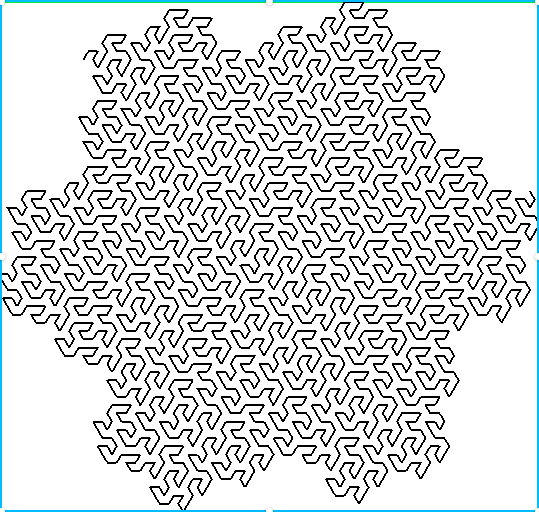
\includegraphics[width=.7\linewidth]{flosnek_4it}
  \caption{4 iterates}
\end{subfigure}%
\begin{subfigure}{.5\textwidth}
  \centering
  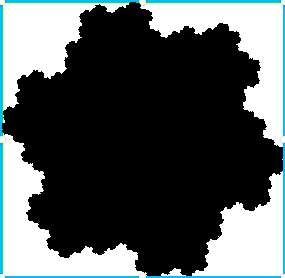
\includegraphics[width=.7\linewidth]{flosnek_8it}
  \caption{8 iterates, rescaled}
\end{subfigure}
\caption{Rendering of \textsc{Gosper's flowsnake}, with \gls{bounding box}}
	\label{fig:flosnek}
\end{figure}

The curve ist generated by iterating a set of substitution rules called \gls{lsys}, which will be described in detail in \ref{somehwhere}.

Furthermore, the presented curve is a \gls{pfc}, as - if the \gls{lsys} substitution is executed an infinte amount of times - it will fill all of the 2D plane without ever intersecting.

\section{Problem Statement}
In 2016, Prof. Jörg Arndt, the supervisor of this thesis, conducted research on finding \gls{pfc}s for \gls{lsys} with one non-constant character and published an article (\cite{Arndt2016}), where he presented 2D renderings of the \gls{pfc}s found.

The tools used to get from an \gls{lsys} description to a graphical, embeddable rendering of the iterated curve were assortments of chained commandline scripts, leaving much to be desired in flexibility and eas-of-use.

Thus, a request was issued for the creation of a \emph{cross-platform, maintainable and extensible} software that is able to create, visualize and export \gls{pfc}s from their \gls{lsys} descriptions.

\section{Approach}

Since this problem is multi-faceted, and the additional requirements introduce significant complexity on top of the "implement a renderer/exporter" core task, a structured approach to finding a solution is taken using decomposition methods from software engineering.

First, the requirements are formulated and discussed.

Then, research is conducted on available technologies for satisfying given requirements.

An architectural model is created using \gls{uml} to define the system architecture.

This model ist then implemented and refined/amended to address issues arising during the implementation process.

The software is tested during development with \gls{ci} and \gls{Unit Testing} techniques.

Finally, a short investigation of application performance is conducted.

\section{Requirements to a Solution}
The following requirements to a satisfactory solution are given in figure \ref{img1}.

\begin{figure}[h]
	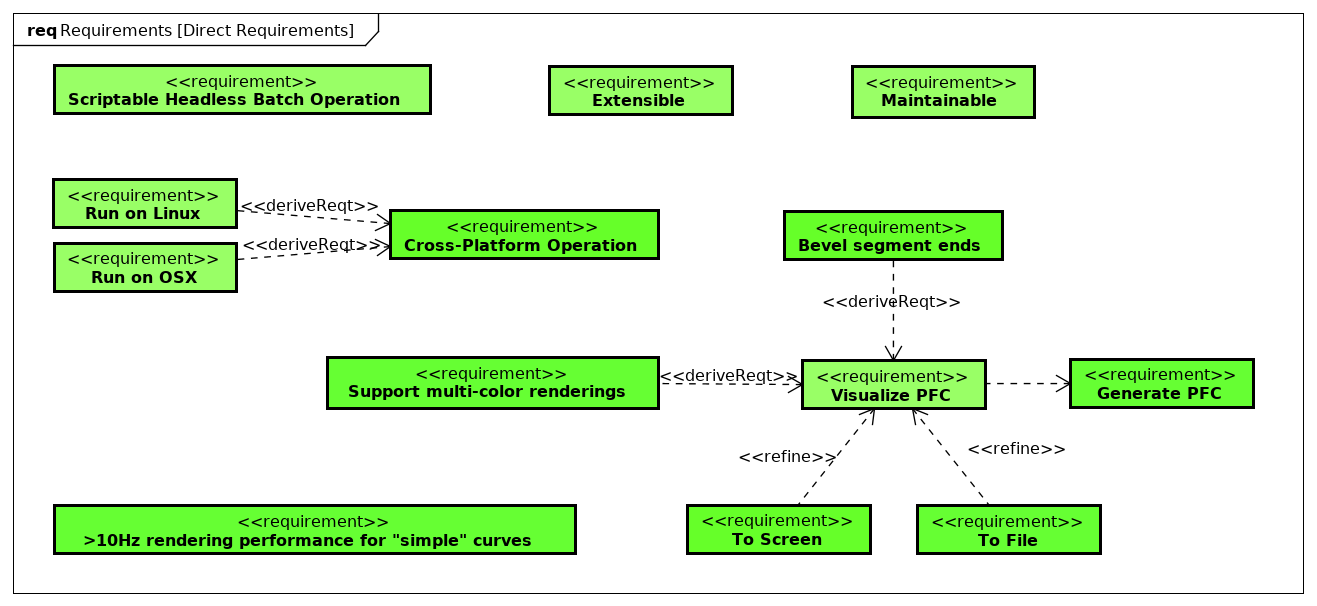
\includegraphics[width=\textwidth]{Intro_DirectRequirements}
	\caption{Direct user requirements to a solution}
	\label{img1}
\end{figure}

These requirements are discussed in detail in the following sections and an architecture is formulated that satisfies them.
